\newcounter{comparison} \setcounter{comparison}{1}

\chapter{Comparison of Results}\label{chapter-comparison}

\begin{abstract}
     This chapter will analyze and compare the results of each method and model variation pairing, according to the comparison metrics established in \cref{dev-comparisons}. In the same way that \cref{dev-comparisons} separated metrics into three main categories, the comparisons will also be discussed in three primary sections. The first, \cref{results-compare-complexity}, will discuss the two identified comparison methods that involve the setup needs for each method. Next, \cref{results-compare-communication} will cover the metrics related to method communication. Finally, the results themselves will be compared in \cref{results-compare-results}. 
\end{abstract}

\newpage

\section{Setup Complexity}\label{results-compare-complexity}
    \subsection{Comparison \thecomparison : Complexity of problem setup}\stepcounter{comparison}
    Based on the definition of this metric in \cref{dev-comparisons}, problem setup involves two components: setup requirements that are identified by method structure and setup requirements specific to the tooling used to perform an analysis. Because the three methods considered in this study are all based on an RDM structure, the requirements for model specification are the same. Each follows the XLRM structure that supports a series of uncertainties and levers connected through relationships to the identified outcomes of interest. Therefore, there is no significant difference in terms of method-required problem setup. 
    
    The second element of problem setup relates to the requirements of any software packages that are used to execute analysis. For example, a tool like OpenMORDM provides a well-structured implementation of the MORDM method, which can also support multi-scenario MORDM, but is not able to support the functionality required for MORO \citep{Hadka2015}. Given that multi-objective robust optimization has not yet been presented as a formal RDM-based method in literature until now, there is no well-structured package similar to OpenMORDM for MORO. 
    
    This study makes use of the Exploratory Modelling and Analysis (EMA) Workbench for all three methods, which provides a highly customization interface with which to implement the steps required for all methods \citep{Kwakkel2017}. This package is not as precisely structured as OpenMORDM, which provides for a higher level of customization and flexibility, but correspondingly requires more work to establish the required configuration. Because this package is able to support all three methods considered in this study, model configuration is similar. The differences lie in the lake problem variations themselves. The EMA Workbench provides native support for several model implementations, including Vensim, NetLogo, and Python, which is the implementation used in this study. The Python implementations require uncertainties and decision levers to be specified as individual parameters of the method function. This process can get unwieldy given a large number of uncertainties and levers, as in the case of the intertemporal lake problem, but is quite straightforward. 
    
    \begin{comparisonbox}{Summary: Complexity of Problem Setup}
        The fact that the methods considered all have a foundation in robust decision making, and that the same software package can be used for each method, means that there is no significant differences in the complexity of problem setup. 
    \end{comparisonbox}

    \subsection{Comparison \thecomparison : Complexity of method setup}\stepcounter{comparison}
    The complexity of method setup refers primarily to the effort involved in steps 2-4 of the RDM process. Because steps 3 and 4 are common to all three methods, setup for these will not be compared here. The difference in each method lies in the policy alternative determination, or search phase, and specifically in two elements of the search phase that make each method unique. 
    
    The first is the manner in which data is gathered to compare potential policy alternatives, which will be referred to as the reference scenario or scenarios. With respect to MORDM, this is quite straightforward: a single predefined reference scenario is used, called the base reference scenario. The work required to setup alternative comparison is also quite straightforward in MORO, where a constant and small ensemble of uncertainty vectors is used throughout the entire search. This only requires a sampling across the uncertainty space that is already defined in model specification. As described in \cref{dev-step2}, Latin Hypercube Sampling was used to build this small ensemble, which is a well-established sampling technique built into EMA Workbench. By leveraging built in sampling functionality, the effort required to set up the alternative comparison component of the search remains quite small for MORO. 
    
    Reference scenario configuration is more complex in multi-scenario MORDM, as this method involves the specification of multiple scenarios that are independently used to locate potentially robust policy alternatives. As discussed in \cref{step2-scenarios}, there are many possible ways to select scenarios. If the analyst decides to use a random set of scenarios selected from a large ensemble of uncertainty settings, or if those scenarios are determined exclusively through decision maker input, the reference scenario selection process does not significantly add to the complexity of setup for multi-scenario MORDM. 
    
    This study uses a significantly more time intensive method of selection that requires the completion of an MORDM analysis before selecting reference scenarios. In the initial MORDM run, scenario discovery is used to determine the boundaries of vulnerability that remain in that discovered set of policy alternatives. Once those boundaries are determined, that information is used to select a set of maximally diverse alternatives from within those boundaries. This involves first building a larger ensemble of uncertainty vectors and selecting those vectors that fall within the vulnerable range. Then, an exhaustive search is used from within the identified group to determine which set of uncertainty vectors are maximally diverse. As this is an exhaustive search, each possible combination of policies must be examined. This process can get extremely computationally expensive very quickly, as indicated by \cref{fig:trend-policycombinations}. As the size of the set of uncertainty vectors with which to select a set of reference scenarios from increases, the number of combinations of maximally diverse policy alternatives grows exponentially. This computational cost has a significant impact on the cost and complexity of the search phase in multi-scenario MORDM. 
    
    \begin{figure}[ht]
        \centering
        \captionsetup{width=0.5\textwidth}
        
        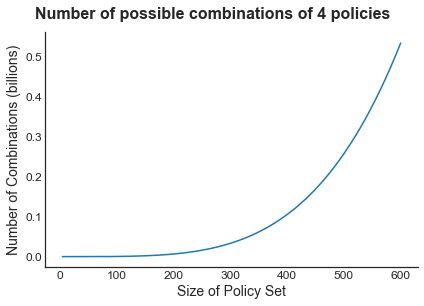
\includegraphics[width=0.5\textwidth]{compare/trend_combinations}
        \caption[Trend in computational cost when selecting maximally diverse policies]{The number of possible combinations of 4 policies given a set of available policies. This demonstrates the rapid increase of combinations and therefore of computational cost when determining maximally diverse scenarios.}
        \label{fig:trend-policycombinations}
    \end{figure}

    The second configuration element of the search phase is the manner in which policies are compared. Both MORDM and multi-scenario MORDM use the same outcome definitions as in the model specification phase, requiring no additional configuration work. MORO requires a custom comparison definition, which depends on the robustness method used. If it involves a comparison to another specific scenario (worst or best case performance, for example), then that worst or best case scenario must be found before the search can begin. If the robustness metric instead looks at performance below a threshold, as in the case of this study, then the comparison definition involves defining how to compare each outcome to the relevant threshold in order to begin the search. 
    
    \begin{comparisonbox}{Summary: Complexity of Method Setup}
        The elements of setup complexity are summarized in \cref{table:setupcomplexity}. This table provides a quick view of the differences in the two interesting elements of configuration for the search phase. The value in parentheses indicates the effort required for this study, specifically. So, for this study, multi-scenario MORDM involves the most complexity with respect to method setup. 
    \end{comparisonbox}
    
    \begin{table}[ht]
        \centering
        \captionsetup{width=0.70\textwidth}
        \caption[Setup Complexity of Methods]{Complexity of configuration in the policy alternative determination phase. Effort provides a qualitative idea of the amount of work required to configure the search, given an already specified model. }
        \label{table:setupcomplexity}
        
        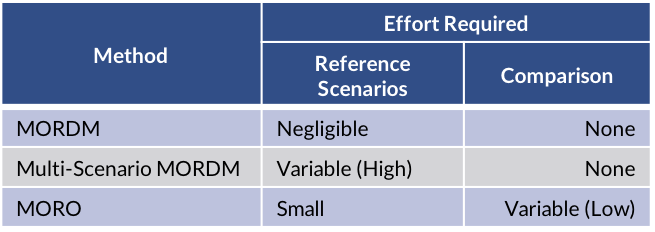
\includegraphics[width=0.7\textwidth]{compare/complexity_table}
    \end{table}
        
\section{Communication}\label{results-compare-communication}
    \subsection{Comparison \thecomparison : Results communication} \stepcounter{comparison}
    As described in \cref{dev-comparisons}, results communication refers to the way in which each method communicates results during execution. In the case of this study, each method considered is following the same RDM-based structure. Correspondingly, results communication is common across each of the methods. For review, the communication of each step is described here. The first step, model specification, involves setup for the following three RDM phases, and so does not involve communication of any results. The end of step 2, policy alternative determination, involves the reporting of the complete set of potentially robust policy alternatives that will be used in the remaining two steps. At this point in the analysis, therefore, analysts and decision makers will know the set of alternatives that has been identified. In the remaining two steps of the analysis, more information about the policy alternatives, including the assessed robustness of each alternative when considering a wide array of potential future states of the world in step 3 and remaining vulnerabilities that the alternatives still have in step 4. 
    
    \begin{comparisonbox}{Summary: Results Communication}
        Results communication is common across all three methods. Policy alternatives are reported in step 2 of each method, the robustness of each alternative is revealed in step 3, and potential vulnerabilities are communicated at the conclusion of step 4, scenario discovery.
    \end{comparisonbox}
    
    \subsection{Comparison \thecomparison : Robustness communication} \stepcounter{comparison}
    Each method, based on the RDM structure, is able to use the same robustness metric to determine policy robustness in the uncertainty analysis stage, so there is no method-specific difference in robustness communication. As this is then dependent on the robustness metric selected, it is not applicable to this study, which is focusing on the impact of selection of a robust decision support method on the analysis process. 
    
    \begin{comparisonbox}{Summary: Robustness Communication}
        The robustness metric used is common across all three methods, and therefore there is no difference in robustness communication for this study. 
    \end{comparisonbox}

    \subsection{Comparison \thecomparison : Ease of results updating if model specification changes} \stepcounter{comparison}
    The impact of a change in model specification will be explored for steps 2-3 of each robust decision support method. Fundamentally, a change in model specification will impact all methods in a similar way, due to the fact that they each follow the same basic RDM structure. The decision about how much of the process should be repeated relates more to decision maker goals, as described below. 
    
    \textbf{Step 2: Policy Alternative Determination}: For every method, a change in method specification will require a complete restart of the search process in the policy alternative determination phase, especially if the analyst or decision makers think that the change will have a significant impact on the resulting set of non-dominated policy alternatives. 
    
    \textbf{Step 3: Uncertainty Analysis}: If decision makers are primarily interested in how these changes will affect the robustness of an existing set of non-dominated policy sets, a specification change need only lead to a new ensemble of uncertainty settings with which to test the efficacy of each policy alternative. Again, this is common to all methods that are being studied here.
    
    \textbf{Step 4: Scenario Discovery}: A change in model specification does not directly result in an alteration to the scenario discovery process. It is impacted through changes to the previous two steps of analysis and must be reran to determine the impact of specification changes on any previously identified vulnerable regions.
    
    \begin{comparisonbox}{Summary: Ease of results updating if model specification changes}
         The impact of a change in the model specification affects all three methods under consideration in the same way. Updates may be required in steps 2 or 3 depending on they type of change and decision maker goals.
    \end{comparisonbox}
    
    \subsection{Comparison \thecomparison : Ease of results updating if robustness metric changes} \stepcounter{comparison}
    The impact of a change in the robustness metric will be explored for steps 2-3 of each robust decision support method. Fundamentally, a change in robustness metric most affects the uncertainty analysis step. However, because MORO directly incorporates robustness into the policy analysis determination process, a change in robustness metric may also force a re-run of that step as well. 
    
    \textbf{Step 2: Policy Alternative Determination}: A change in robustness metric will have no impact on this step for MORDM. Because the MORO method incorporates robustness into the search process, if the change relates to the definition of robustness used to sort policy alternatives, a change in robustness metric demands that the search process be repeated. 
    
    It is also possible that a change in robustness metric will impact multi-scenario MORDM. Because such a change may affect what is identified as a vulnerable region in the scenario discovery process of an MORDM analysis, the range with which to select a set of reference scenarios from may change for the multi-scenario MORDM analysis. Such a change would require a complete restart of the search process for each newly identified reference scenario.
        
    \textbf{Step 3: Uncertainty Analysis}: For all methods, a change in the robustness metric will not force a repeat of the computational exploration phase of uncertainty analysis, which simply builds a large data set that indicates the performance of each policy alternative over a wide range of potential states of the world. A change in the robustness metric would require recalculation of the robustness of each policy at this stage for each decision support method. 
    
    \textbf{Step 4: Scenario Discovery}: This step will be directly affected by a change in robustness metric if that change results in a different definition of which policy and uncertainty sets lead to "interesting" outcome values. For example, in the case of a domain criterion metric, a change in threshold value may affect how "interesting" data points are identified. For the most part, though, scenario discovery will be repeated based on changes in the search phase or uncertainty analysis. 

    \begin{comparisonbox}{Summary: Ease of results updating if robustness metric changes}
        As the robustness metric is common for all three methods, a change in robustness metric requires the recalculation of the robustness of each policy alternative in Step 2: Uncertainty Analysis for all. Furthermore, because MORO uses robustness to compare policy alternatives in the search phase, a change in the definition of robustness there will require a total restart of the search phase. 
    \end{comparisonbox}

\section{Results}\label{results-compare-results}
    \subsection{Comparison \thecomparison : Computational cost} \stepcounter{comparison}
    The comparison of computational cost will primarily consider the number of model executions required to complete the policy alternative determination step of each method. Also discussed is the computational cost of uncertainty analysis, which revolves around the number of model evaluations required to build the complete data set of experiments (where an experiment is the sets of uncertainty and lever values, and associated outcomes of interest). 
    
    \begin{table}[t!]
    \captionsetup{width=\textwidth}
    \caption[Computational cost for all pairings]{Computational cost determined for each model variation and method pairing. Total computational cost, calculated as number of model function executions, can be found in the last rows.}
        
    \begin{subtable}{\textwidth}
        \centering
        \captionsetup{width=\textwidth}
        \caption{Step 2: Policy Alternative Determination}
        \label{table:computationalcost}
        
        \rowcolors{2}{odd-row-blue}{even-row-blue}
        \setlength\arrayrulewidth{1pt}\arrayrulecolor{white}
        \begin{tabularx}{\textwidth}{l|l|R|R|R}
            \hline
            \rowcolor{tudelft-dark-blue!80}
            \multicolumn{2}{l|}{\color{white} \textbf{}} 
            & \multicolumn{1}{c|}{\color{white} \textbf{MORDM}} 
            & \multicolumn{1}{c|}{\color{white} \textbf{\begin{tabular}[c]{@{}c@{}}Multi-\\ Scenario \\ MORDM\end{tabular}}}
            & \multicolumn{1}{c}{\color{white} \textbf{MORO}} \\ \hline
            
            \cellcolor{even-row-blue}   & Intertemporal    & 500,000   & 500,000  &  300,000    \\ \cline{2-5} 
            \cellcolor{even-row-blue}   & \cellcolor{odd-row-blue}Planned Adaptive &
            \cellcolor{odd-row-blue}100,000   & \cellcolor{odd-row-blue}100,000  & \cellcolor{odd-row-blue}100,000     \\ \cline{2-5} 
            \multirow{-3}{*}{\cellcolor{even-row-blue}\begin{tabular}[c]{@{}l@{}}Number of \\ Function \\ Executions (NFE)\end{tabular}} & DPS             & 100,000   & 100,000  & 100,000      \\ \hline
            
            \multicolumn{2}{l|}{\cellcolor{odd-row-blue}Per Policy Executions} & 1 & 1 & 50 \\ \hline
            \multicolumn{2}{l|}{\cellcolor{even-row-blue}Search Repetitions} & 1 & 5 & 1 \\
            
            \noalign{\global\arrayrulewidth=4pt} \arrayrulecolor{tudelft-dark-blue!80}
            \hline
            \noalign{\global\arrayrulewidth=1pt} \arrayrulecolor{white}
            
            \cellcolor{odd-row-blue}    
            & \textbf{Intertemporal}    & 500,000  & 2,500,000 & 15,000,000  \\ \cline{2-5} 
            \cellcolor{odd-row-blue} 
            & \cellcolor{even-row-blue}\textbf{Planned Adaptive} & \cellcolor{even-row-blue}100,000  & \cellcolor{even-row-blue}500,000   & \cellcolor{even-row-blue}5,000,000    \\ \cline{2-5} 
            \multirow{-3}{*}{\cellcolor{odd-row-blue}\textbf{\begin{tabular}[c]{@{}l@{}}Computational \\ Cost (NFE)\end{tabular}}}
            & \textbf{DPS}              & 100,000  & 500,000   & 5,000,000           \\ \hline
        \end{tabularx}
    \end{subtable}
    \newline
    \vspace*{0.3 cm}
    \newline
    \begin{subtable}{\textwidth}
        \centering
        \captionsetup{width=\textwidth}
        \caption{Step 3: Uncertainty Analysis}
        \label{table:cost-uncertainty}
        
        \rowcolors{2}{odd-row-blue}{even-row-blue}
        \setlength\arrayrulewidth{1pt}\arrayrulecolor{white}
        \begin{tabularx}{\textwidth}{l|l|R|R|R}
            \rowcolor{tudelft-dark-blue!80}
            \multicolumn{2}{l|}{\color{white} \textbf{}} 
            & \multicolumn{1}{c|}{\color{white} \textbf{MORDM}} 
            & \multicolumn{1}{c|}{\color{white} \textbf{\begin{tabular}[c]{@{}c@{}}Multi-\\ Scenario \\ MORDM\end{tabular}}}
            & \multicolumn{1}{c}{\color{white} \textbf{MORO}} \\ \hline
            
            \cellcolor{even-row-blue}   & Intertemporal  & 90 & 291 & 7 \\ \cline{2-5} 
            \cellcolor{even-row-blue}   & \cellcolor{odd-row-blue}Planned Adaptive &
            \cellcolor{odd-row-blue}48   & \cellcolor{odd-row-blue}113  & \cellcolor{odd-row-blue}6     \\ \cline{2-5} 
            \multirow{-3}{*}{\cellcolor{even-row-blue}\begin{tabular}[c]{@{}l@{}}Number of \\ Nondomianted \\ Alternatives\end{tabular}} & DPS             & 110 & 209 & 22 \\ \hline
            
            \multicolumn{2}{l|}{\cellcolor{odd-row-blue}Uncertainty Ensemble Size} & 10,000 & 10,000 & 10,000 \\
            
            \noalign{\global\arrayrulewidth=4pt} \arrayrulecolor{tudelft-dark-blue!80}
            \hline
            \noalign{\global\arrayrulewidth=1pt} \arrayrulecolor{white}
            
            \cellcolor{even-row-blue}   & Intertemporal  & 900,000 & 2,910,000 & 70,000 \\ \cline{2-5} 
            \cellcolor{even-row-blue}   & \cellcolor{odd-row-blue}Planned Adaptive &
            \cellcolor{odd-row-blue}480,000   & \cellcolor{odd-row-blue}1,130,000  & \cellcolor{odd-row-blue}60,000     \\ \cline{2-5} 
            \multirow{-3}{*}{\cellcolor{even-row-blue}\textbf{\begin{tabular}[c]{@{}l@{}}Computational \\ Cost (NFE)\end{tabular}}} & DPS             & 1,100,000 & 2,090,000 & 220,000 \\ \hline
        \end{tabularx}
    \end{subtable}
    \end{table}
    
    A catalog of the computational cost for the search phase can be found in \cref{table:computationalcost}. The results indicate that methods that more directly include robustness considerations incurr a larger computational cost in the search phase of analysis. Given the configuration details used, multi-scenario MORDM is 5 times more expensive than MORDM (because 5 scenarios are considered here), and MORO is 50 times more expensive, based on the use of an ensemble of 50 uncertainty settings in the search process. Therefore, computational cost in this step seems to incorporate a trade-off between efficiency and robustness. 
    
    There is also a variation in computational cost in step 3, based on the size of each set of non-dominated policy alternatives. As \cref{table:cost-uncertainty} indicates, multi-scenario MORDM appears to have the largest computational cost in uncertainty analysis due to the larger number of non-dominated alternatives identified through 5 separate reference scenarios.
    
    The translation of computational cost to physical processing time is not consistent for both steps. There is additional work outside of model execution in the search phase that also contribute to processing time. The MOEA used in this study involves a non-dominated epsilon sort after every generation. This sorting stage takes more time with larger sets of non-dominated alternatives, due to the need for more comparisons each time. It does still contribute a smaller fraction to the total processing time than model execution, so despite sorting taking longer for MORDM due to the larger sets of non-dominated solutions, the overall search process for MORO still takes much longer in total. The uncertainty analysis does not have the same addition of processing time, so physical processing time will be less per model execution
    
    \begin{comparisonbox}{Summary: Computational cost}
        Analysis using MORO has a significantly higher computational cost when compared to the other two methods. Because multi-scenario MORDM involves repeating an MORDM analysis the number of times equal to the number of reference scenarios used (in this case 5), multi-scenario MORDM is also more computational expensive than MORDM. 
    \end{comparisonbox}

    \subsection{Comparison \thecomparison : Convergence of search} \stepcounter{comparison}
    Convergence of an MOEA-based search, as discussed in \cref{results-convergence}, tracks the stabilization of the search for policy alternatives. \cref{fig:compare-convergence} directly compares the epsilon progress and hypervolume convergence trends of each method for a specific model variation. In these plots, a single line represents the mean across all repetitions of the search for each method. In the case of multi-scenario MORDM, each line of the color shown in the legend represents the search for one of the reference scenarios used. For clarity, the multi-scenario MORDM search involving the base reference scenario is left out, as its convergence matches convergence of the MORDM-based search.
    
    There is a difference in mean hypervolume convergence for the intertemporal + MORO pairing as compared to the other two methods. Both epsilon progress and hypervolume stabilize more slowly. This indicates that the minimum number of function executions to ensure stability is higher when using the MORO method for the intertemporal lake problem. It is possible that difference is due to the small size of the set of non-dominated alternatives (6) as compared to the number of decision levers involved (100). The hypervolume of such a small set of alternatives with so many levers can be more significantly impacted by additions or alterations to the set. Furthermore, as changes hypervolume indicate that new policies are being added to the set of non-dominated alternatives, it follows that epsilon progress will have a similarly slower time to convergence. 
    
    The other data point of interest is the epsilon progress of the MORDM-based search with respect to the DPS lake problem variation. Though the epsilon progress here seems to stabilize much more slowly, because the hypervolume convergence is not significantly different, the search process does not seem to be adding policy alternatives that increase the diversity of the non-dominated policy set. When a newly found alternative does not increase diversity of the non-dominated set, no significantly different alternative courses of action are being added to consideration. Therefore, the difference in epsilon progress can be discounted and the stabilization of hypervolume convergence with respect to the DPS + MORDM pairing would seem to have a similar rate of stabilization to the other two pairings involving the DPS model variation. 
    
    There is no significant difference in the convergence of an MOEA-based search when considering the planned adaptive DPS model variation. Each of the methods stabilize at a similar point in the search process in this case. This indicates that no method considered in this study is able to analyze the planned adaptive DPS model with more efficiency than the others. 
    
    \begin{figure}[t!]
        \centering
        \captionsetup{width=\textwidth}
        
        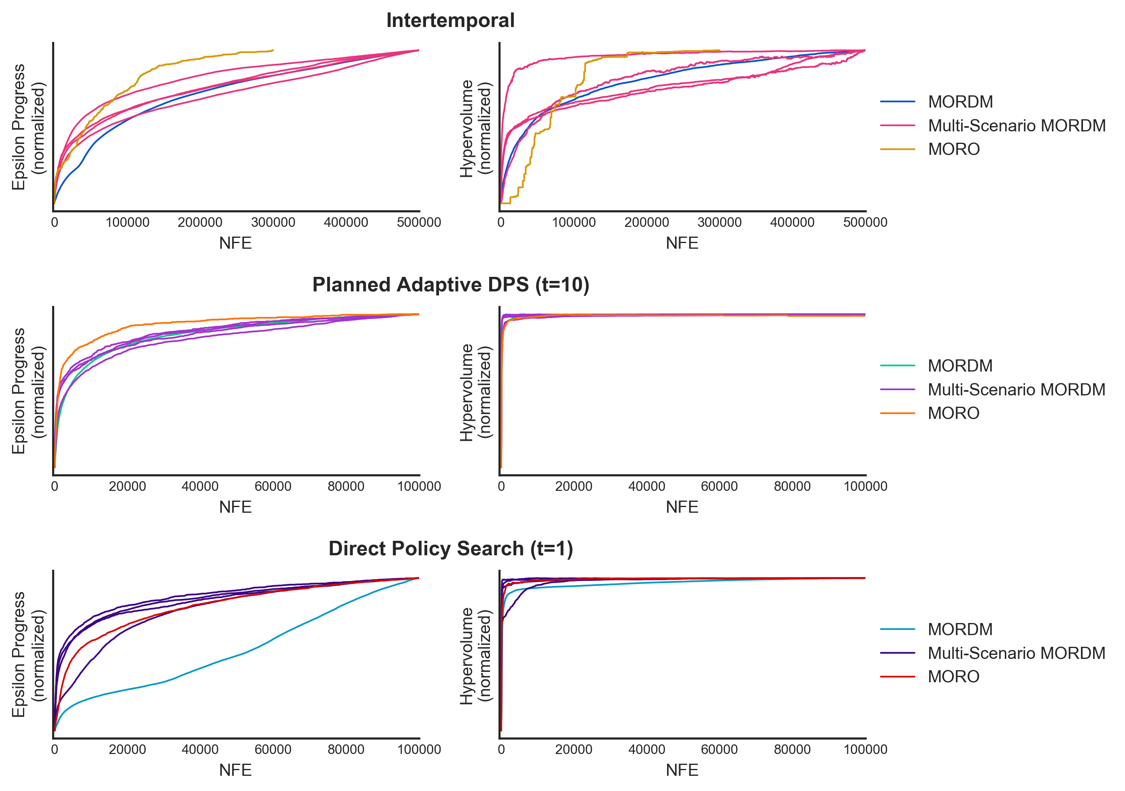
\includegraphics[width=\textwidth]{compare/convergence_normalized}
        \caption[Mean epsilon progress across all pairings and search repetitions]{Mean epsilon progress and hypervolume convergence per model variation and method pairing. Normalized with respect to the maximum value within an individual search process.}
        \label{fig:compare-convergence}
    \end{figure}
    
    \begin{comparisonbox}{Summary: Convergence of search}
        In the case of the planned adaptive DPS model variation, search convergence is very similar across all three methods. The same can be said for the DPS variation, given that the epsilon progress differences for the MORDM method appear to not lead to an increased diversity of the non-dominated set of alternatives, and therefore do not uncover previously unknown combinations of potentially robust decision lever settings. Finally, MORO seems to stabilize more slowly for the intertemporal variation, possibly due to the combination of a large number of decision levers and small size of set of the non-dominated policy alternatives. 
    \end{comparisonbox}
    
    \subsection{Comparison \thecomparison : Robustness of recommended policy set} \stepcounter{comparison}
    As a reminder, this comparison involves examining the overall robustness values for each model variation and method pairing. \cref{fig:robust-heatmap-mean} shows an overall picture of the mean robustness values for each outcome of interest across pairings.
    
    \begin{figure}[ht]
        \centering
        \captionsetup{width=0.8\textwidth}
        
        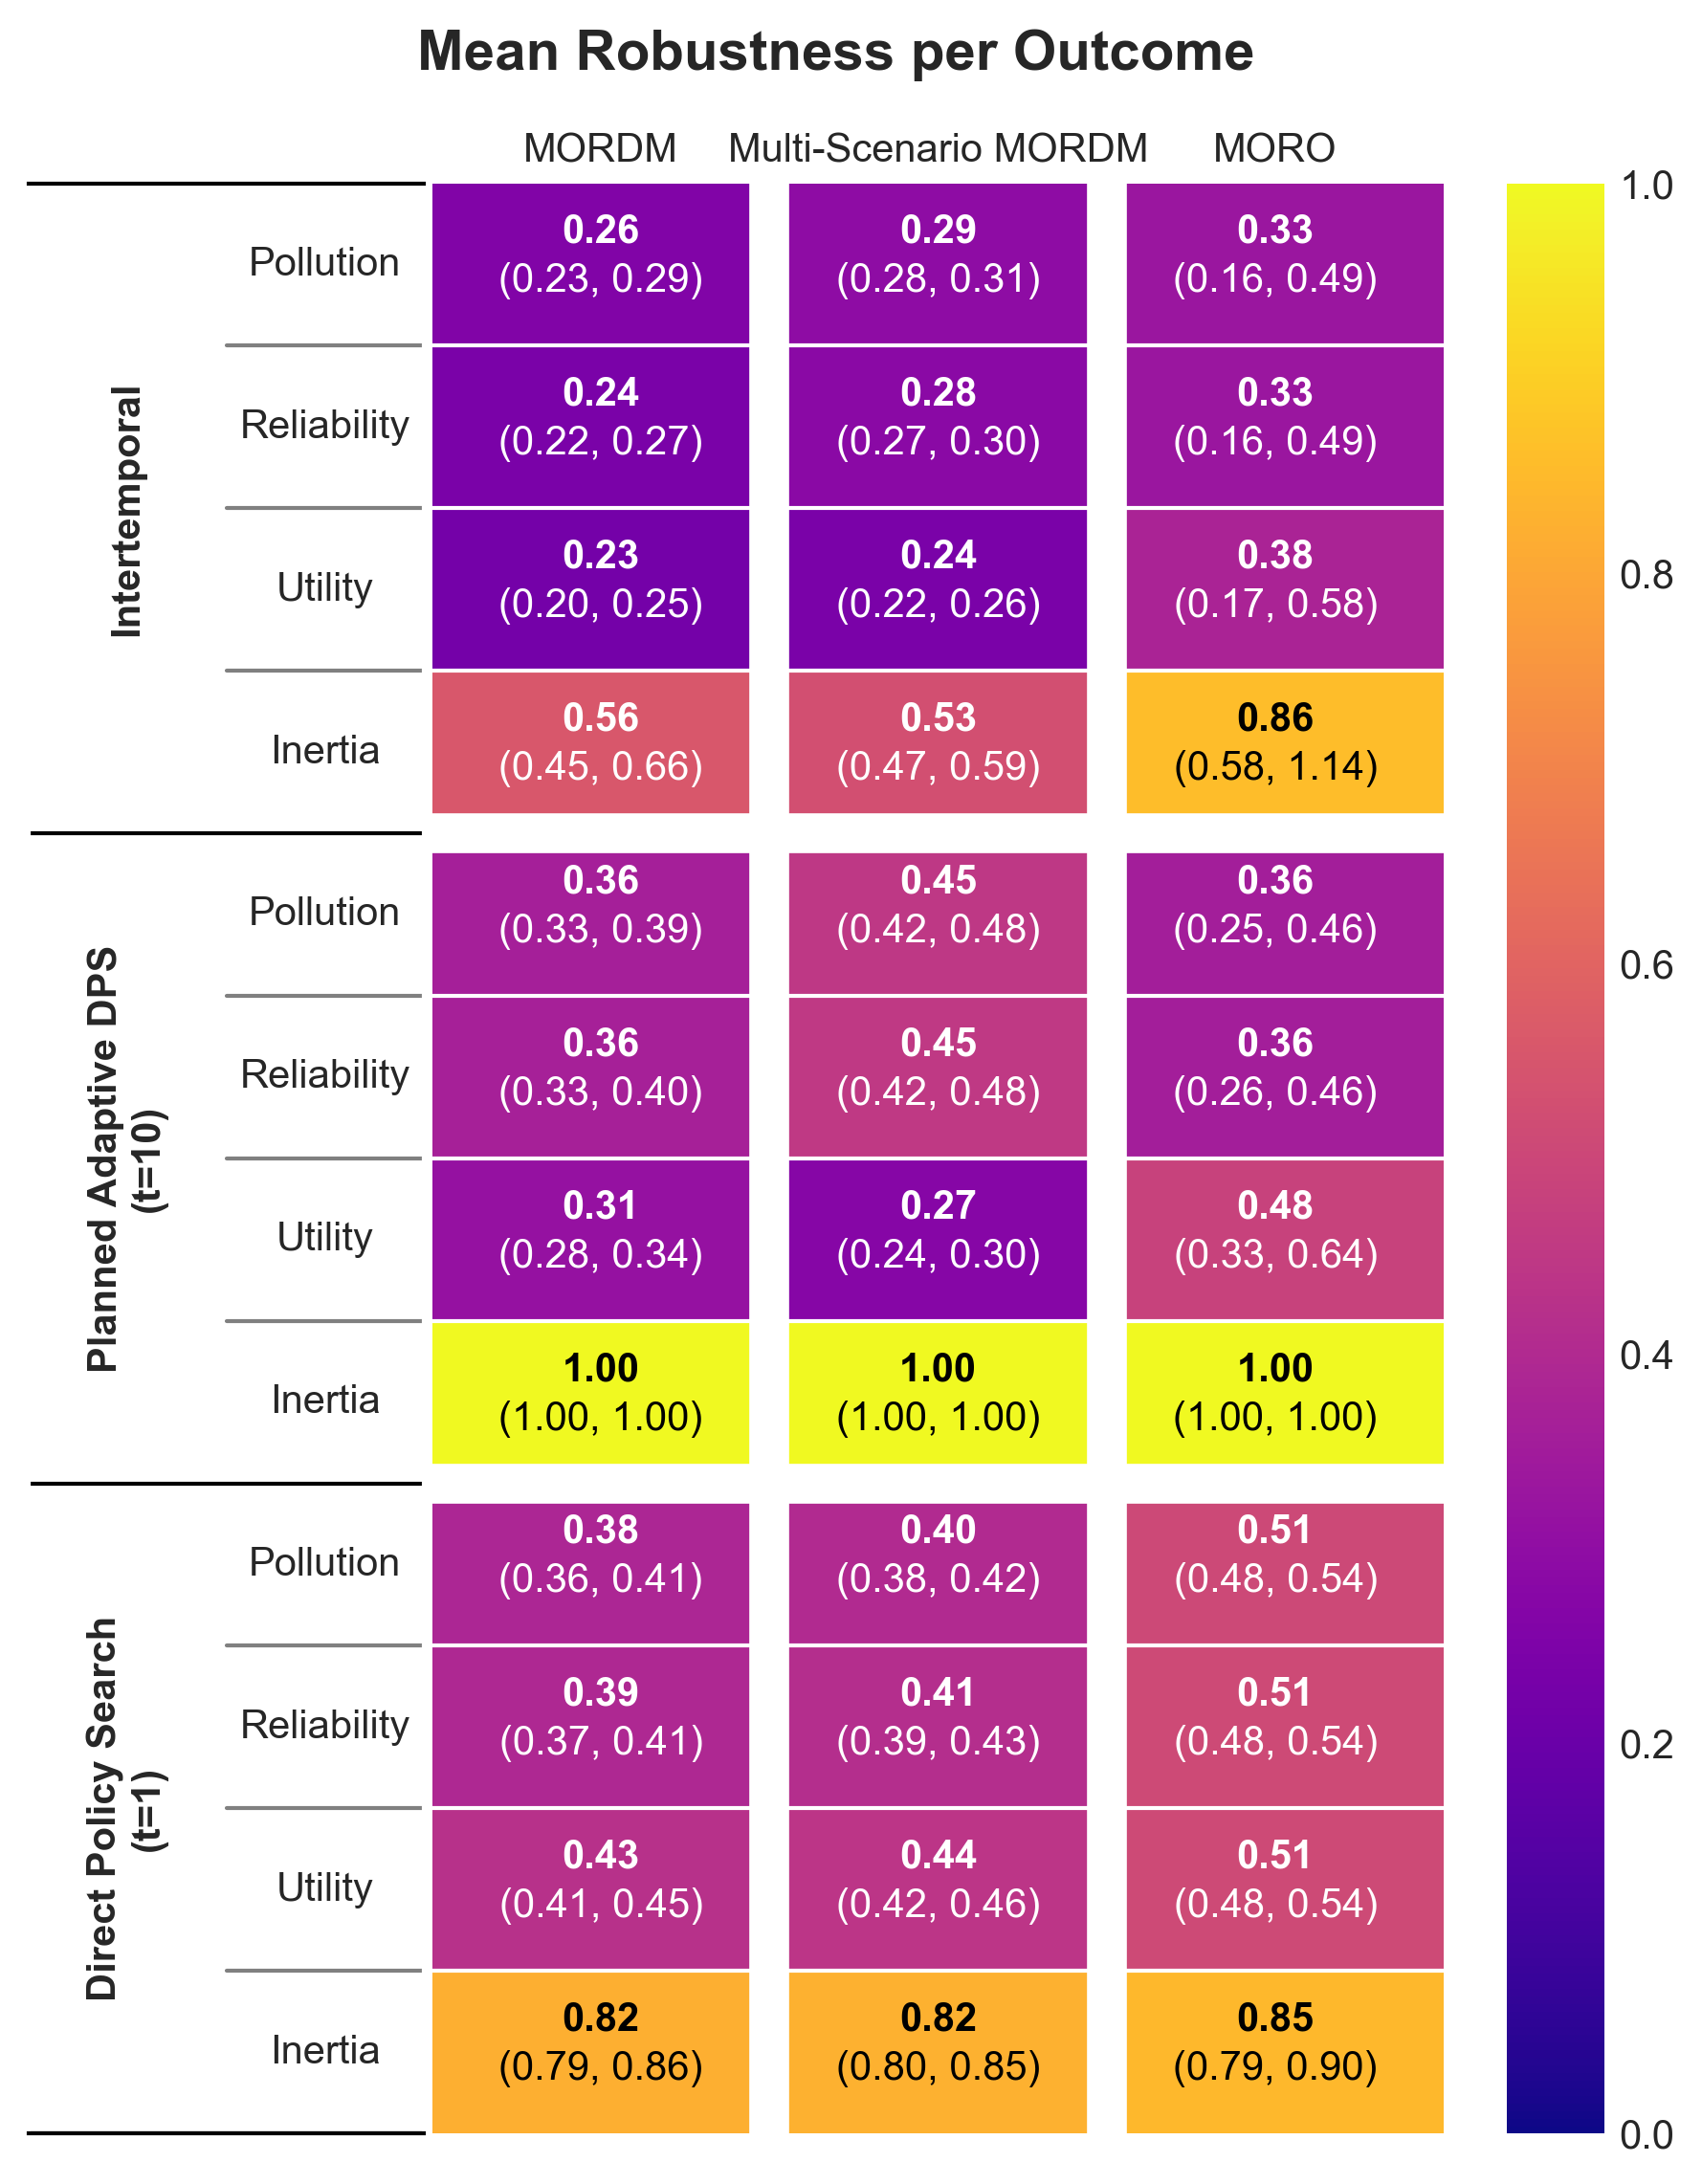
\includegraphics[width=0.8\textwidth]{compare/robust_heatmap_mean}
        \caption[Heatmap of mean robustness across all pairings.]{Mean robustness per model variation and method pairing. This heat map is annotated to include the bounds of the 95 percent confidence interval surrounding the mean.}
        \label{fig:robust-heatmap-mean}
    \end{figure}
    
    The intertemporal and DPS model variations show a general trend of increasing mean robustness from MORDM to MORO, which confirms that the more robustness is incorporated into the search process, the more robust the resulting policy alternatives will be. 
    
    Unlike the intertemporal and DPS model variations, however, the planned adaptive DPS variation shows a sharp increase in robustness of pollution level and reliability, along with a drop in utility from MORDM to multi-scenario MORDM. No increase in robustness of pollution and reliability is seen with respect to the MORDM and MORO methods, also unlike the results seen with the other two variations. Inertia remains constant in this case, with perfect robustness. This result is expected because inertia relates to the consistency of the release decision, and as the release decision changes only every 10 time steps in the planned adaptive DPS variation, inertia of those policies will be high. 
    
    Given that there seems to be an inverse relationship between the pollution or reliability outcomes and utility, it is expected that an increase in the robustness of the first two is associated with a decrease in robustness of the last (\cref{results-step3}). The question then becomes a matter of what caused the change in behavior of robustness in the case of the planned adaptive DPS model variation. 
    
    Examining the release rules that are configured using decision lever values sheds some light onto the potential reason for the different robustness behavior in the case of the planned adaptive DPS model. \cref{fig:release-rules} plots the release rules of the non-dominated policy alternatives for both the DPS and planned adaptive DPS variations and for all three robust decision support methods. These rules show the amount of pollution that would be released for a variety of existing pollution concentrations, as defined by \cref{eq:release-rules} \citep{Quinn2017}. 
    
    \begin{equation}\label{eq:release-rules}
        \alpha_{t} = \frac{X_{t-1}^{q}}{(1+X_{t-1}^{q})} - b*X_{t}
    \end{equation}
    
    \begin{figure}[ht]
        \centering
        \captionsetup{width=\textwidth}
        
        \begin{subfigure}[b]{\textwidth}
            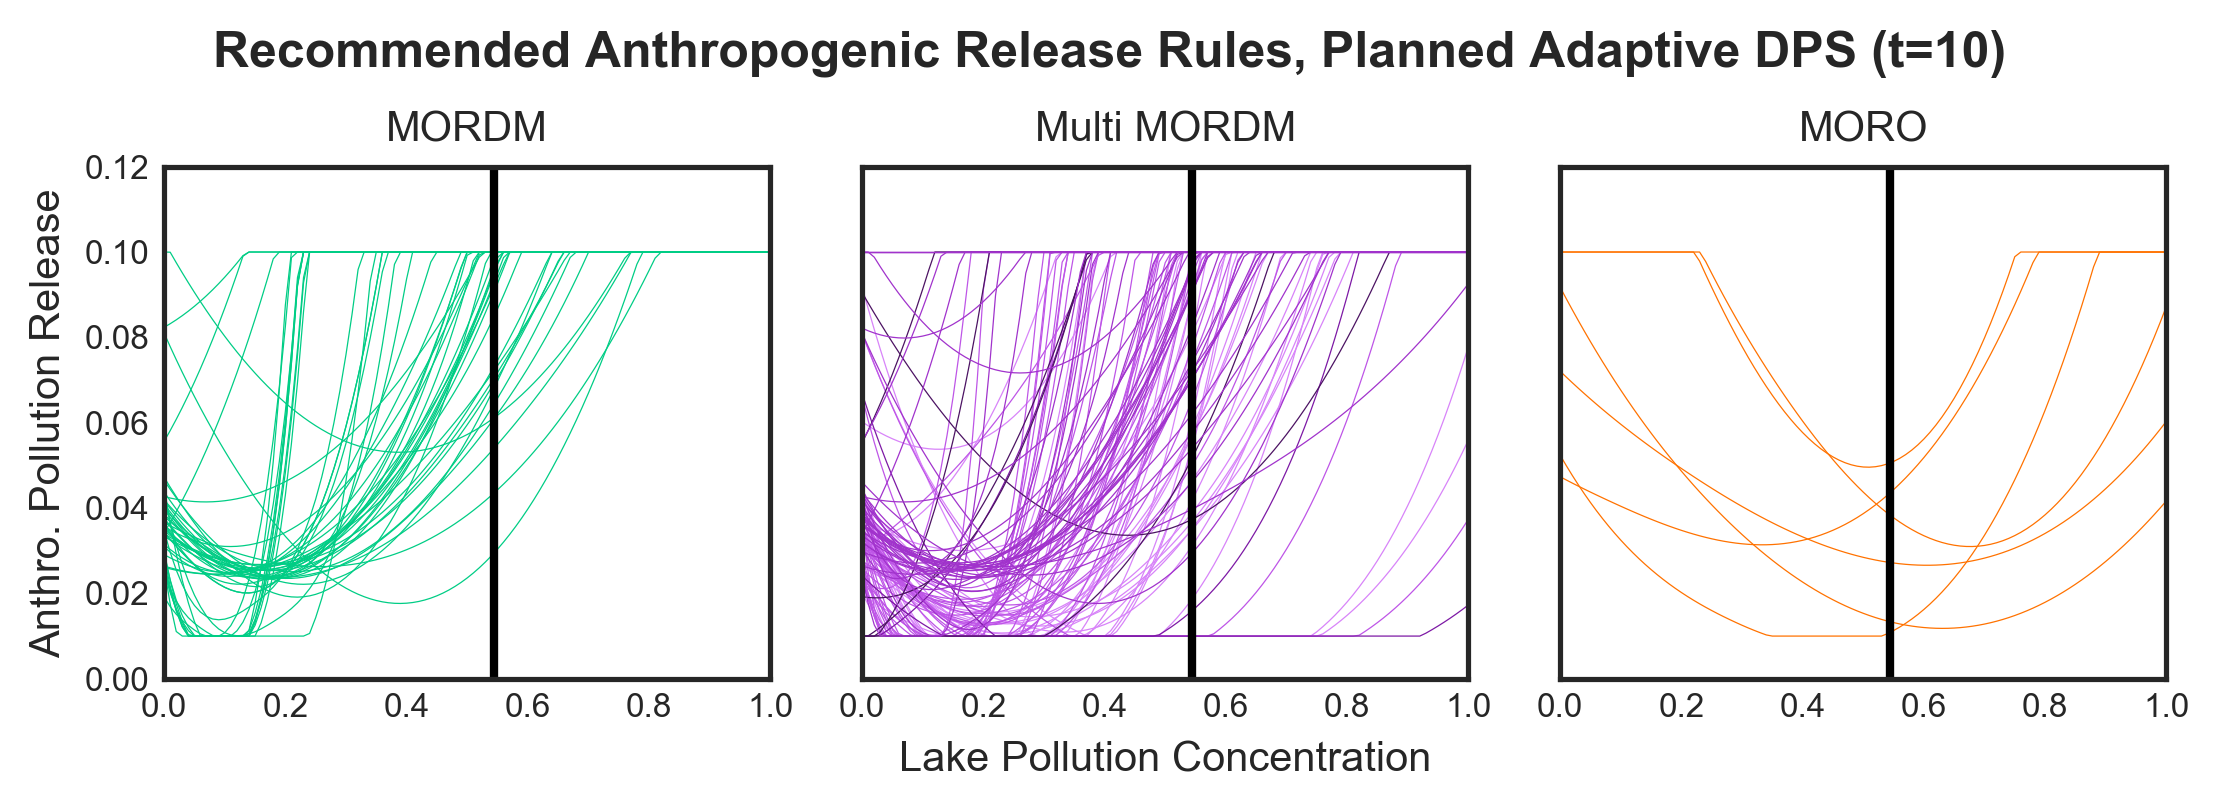
\includegraphics[width=\textwidth]{compare/rules_plannedadaptive_highres}
            \label{fig:planned-releaserules}
        \end{subfigure}
    
        \begin{subfigure}[b]{\textwidth}
            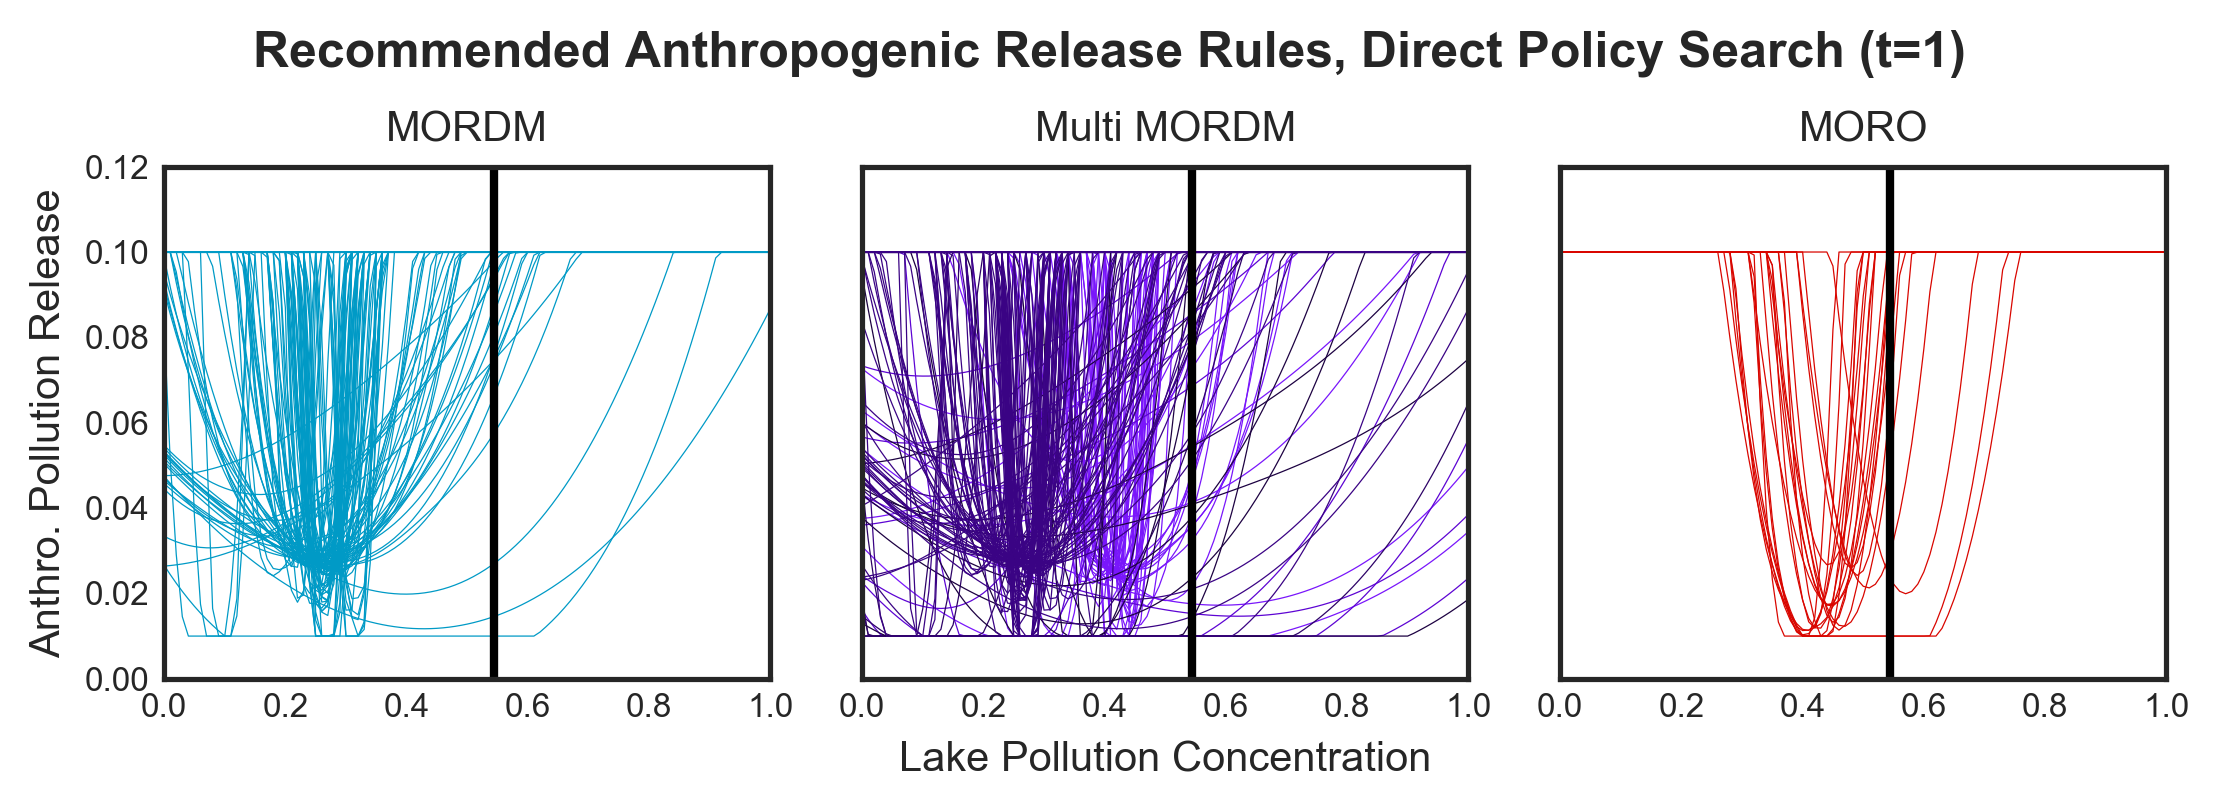
\includegraphics[width=\textwidth]{compare/rules_dps_highres}
            \label{fig:dps-releaserules}
        \end{subfigure}
        
        \caption[Release rules for DPS and planned adaptive DPS variatons]{Release rules for the DPS and Planned Adaptive DPS model variations. The vertical black line indicates the critical pollution level for the reference uncertainty settings (b=0.42, q=2.0).}
        \label{fig:release-rules}
    \end{figure}

    This information indicates that the policy alternatives found through a Multi-MORDM search, especially, produce much more conservative pollution release decisions when compared to the DPS variation, indicated by the pollution concentration which triggers the minimum pollution release amount (which is lower in the planned adaptive DPS variation). The more conservative policy selection would contribute to higher robustness in pollution level and reliability, as well as lower utility robustness, which is what is seen in \cref{fig:robust-heatmap-mean}. 
    
    \begin{figure}[H]
        \begin{subfigure}[b]{\textwidth}
            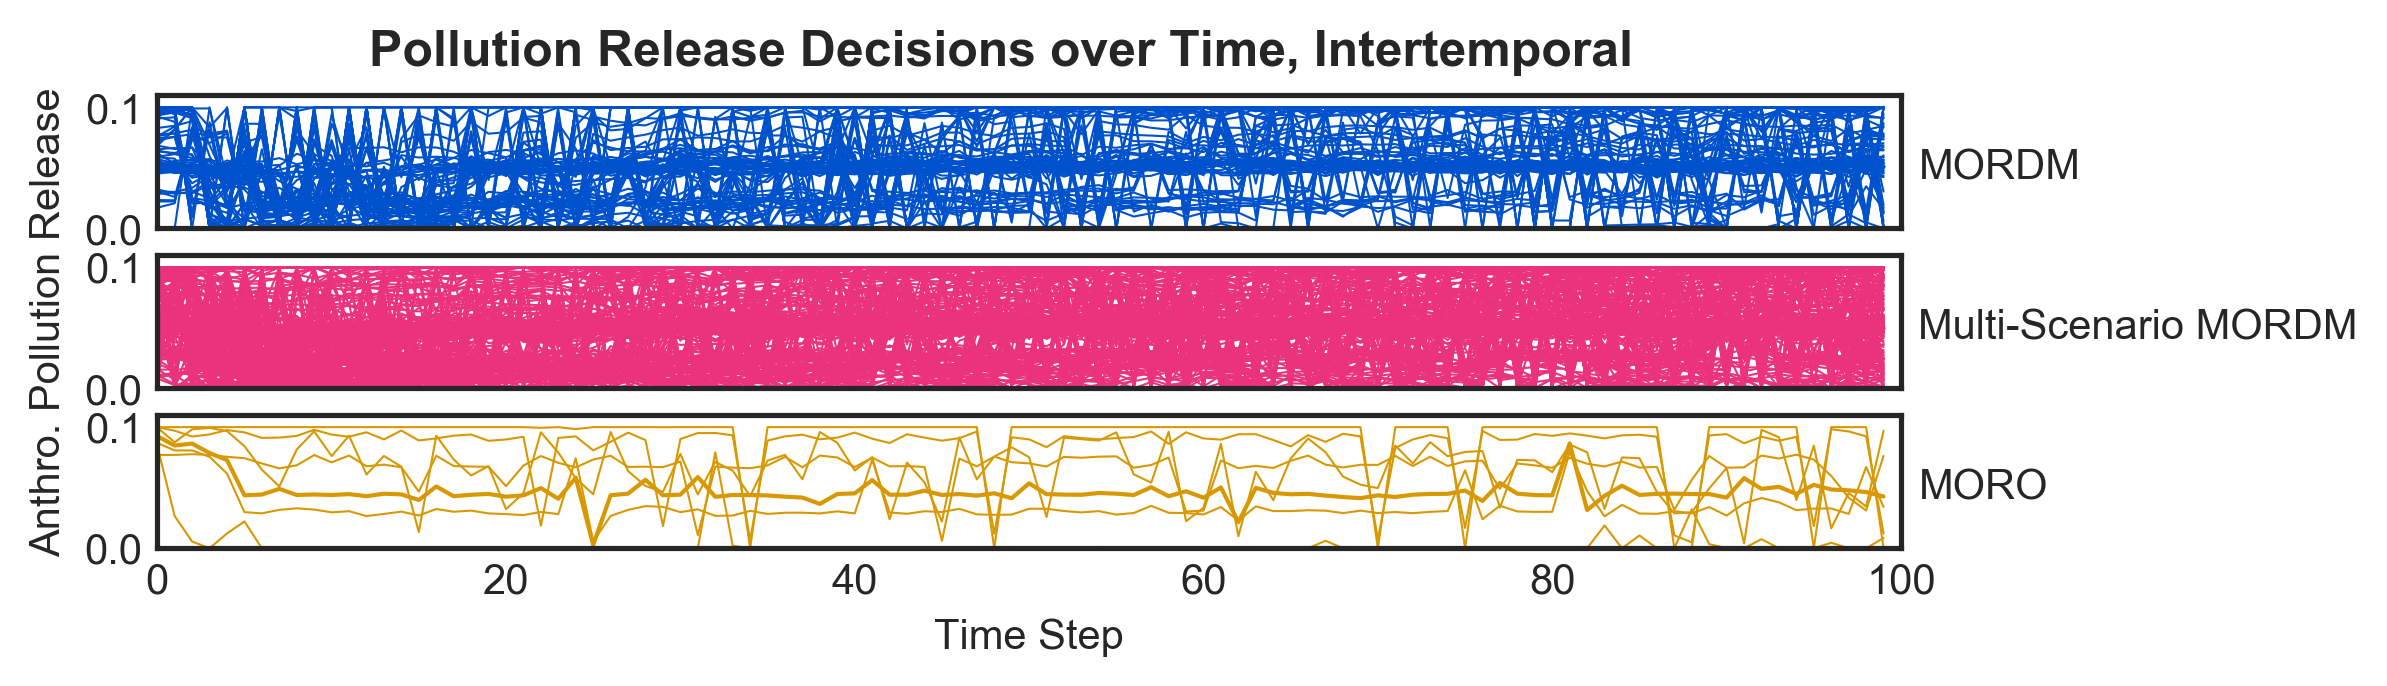
\includegraphics[width=\textwidth]{compare/overtime_intertemporal_highres}
            \label{fig:intertemporal-overtime}
        \end{subfigure}
        \begin{subfigure}[b]{\textwidth}
            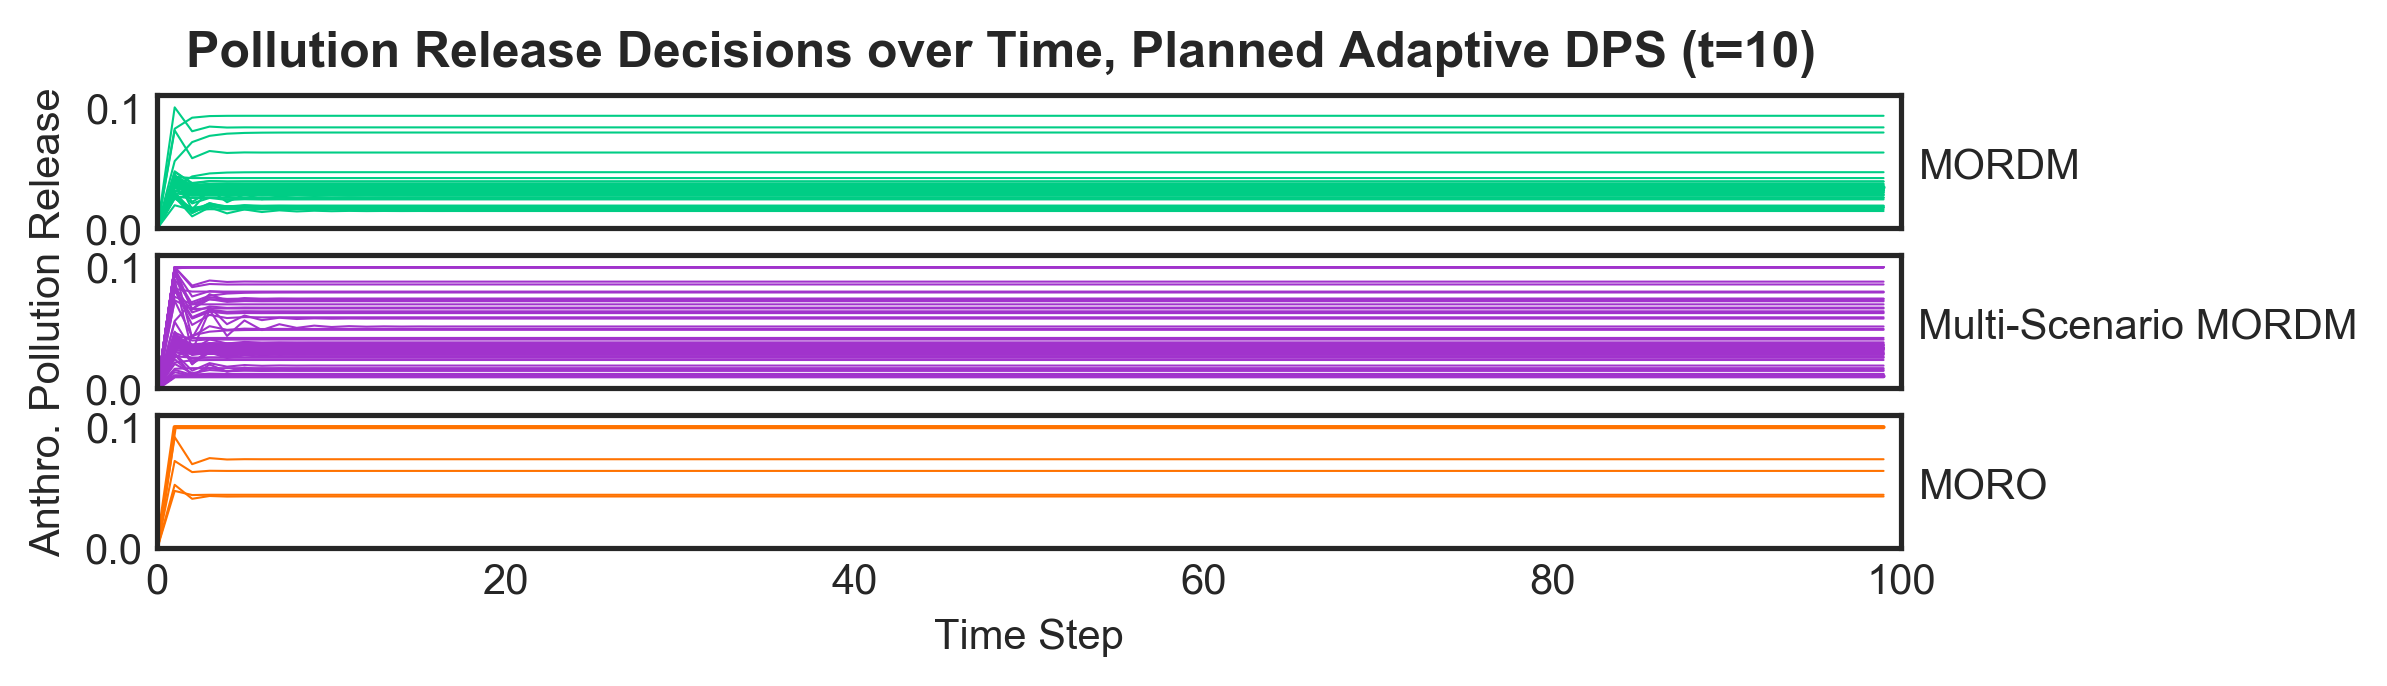
\includegraphics[width=\textwidth]{compare/overtime_plannedadaptive_highres}
            \label{fig:planned-overtime}
        \end{subfigure}
        \begin{subfigure}[b]{\textwidth}
            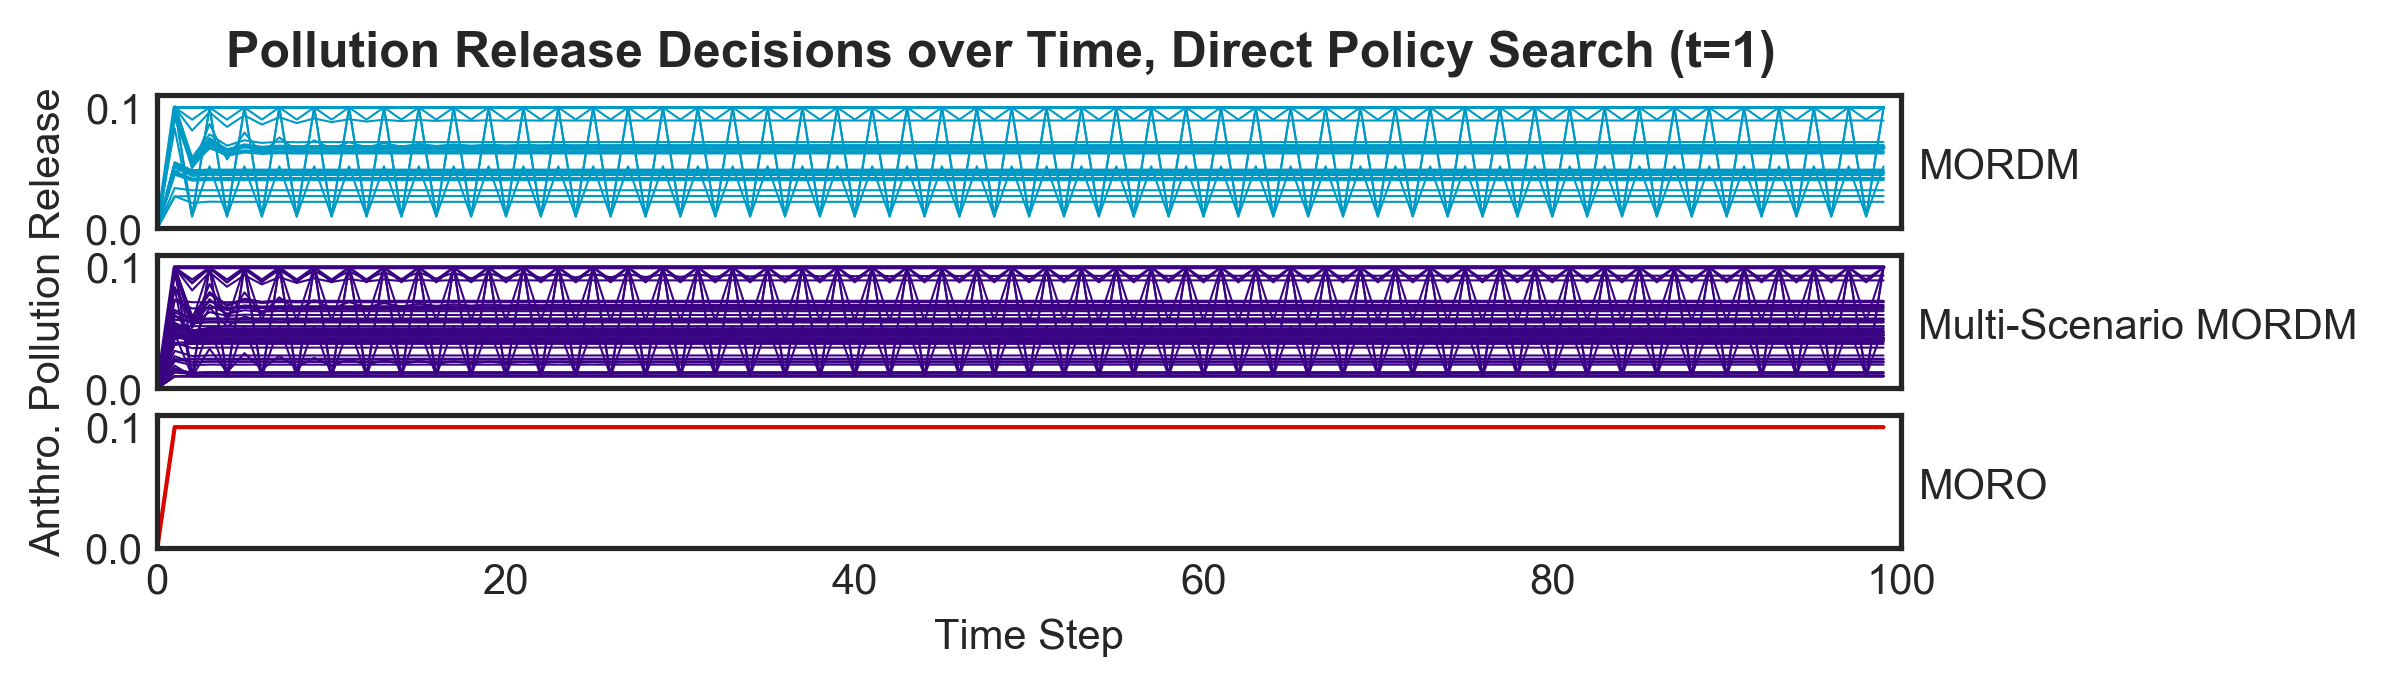
\includegraphics[width=\textwidth]{compare/overtime_dps_highres}
            \label{fig:dps-overtime}
        \end{subfigure}
        
        \caption[Trends in pollution release over time for all pairings]{Trends in pollution release over time of each policy alternative for each model variation and method pairing, assuming base reference scenario uncertainty settings and a starting pollution level of 0.}
        \label{fig:pollution-release-overtime}
    \end{figure}

    The more conservative approach may be driven by the nature of the planned adaptive DPS lake problem, which does not allow for as responsive of decision making as the DPS variation, which can adjust the release amount at every time step, or the intertemporal lake problem, which can also have different release amounts every time period. The anthropogenic pollution release amount over time for identified policy alternatives, shown in \cref{fig:pollution-release-overtime}, as well as the inertia-based robustness values, support this conclusion. The pollution release levels for the planned adapitve DPS lake problem always reach a steady release level, and do so quite quickly, while the other to variations involve frequently changing pollution release amounts over time.

    This trend may also be due to the reference scenarios that were selected for the multi-scenario search phase of the planned adaptive DPS lake problem. To test this theory, a random set of policy alternatives were generated, which were then used in a new multi-scenario MORDM analysis. This lead to a group of policy alternatives, with the mean robustness after uncertainty analysis shown in \cref{fig:robust-heatmap-planned-random}. Comparing robustness values of a random set of reference scenarios to the values generated using the primary set of scenarios generated following the process described in \cref{step2-scenarios} indicates that the selection of reference scenarios has a significant impact on the robustness of policy alternatives. Also, the fact that a random selection of reference scenarios produced robustness similar to MORDM results suggests that the spike in robustness for pollution and reliability (and corresponding drop in utility robustness) is primarily associated with the reference scenario selection and not with any characteristics of the model variation itself. 
    
    \begin{figure}[H]
        \centering
        \captionsetup{width=0.85\textwidth}
        
        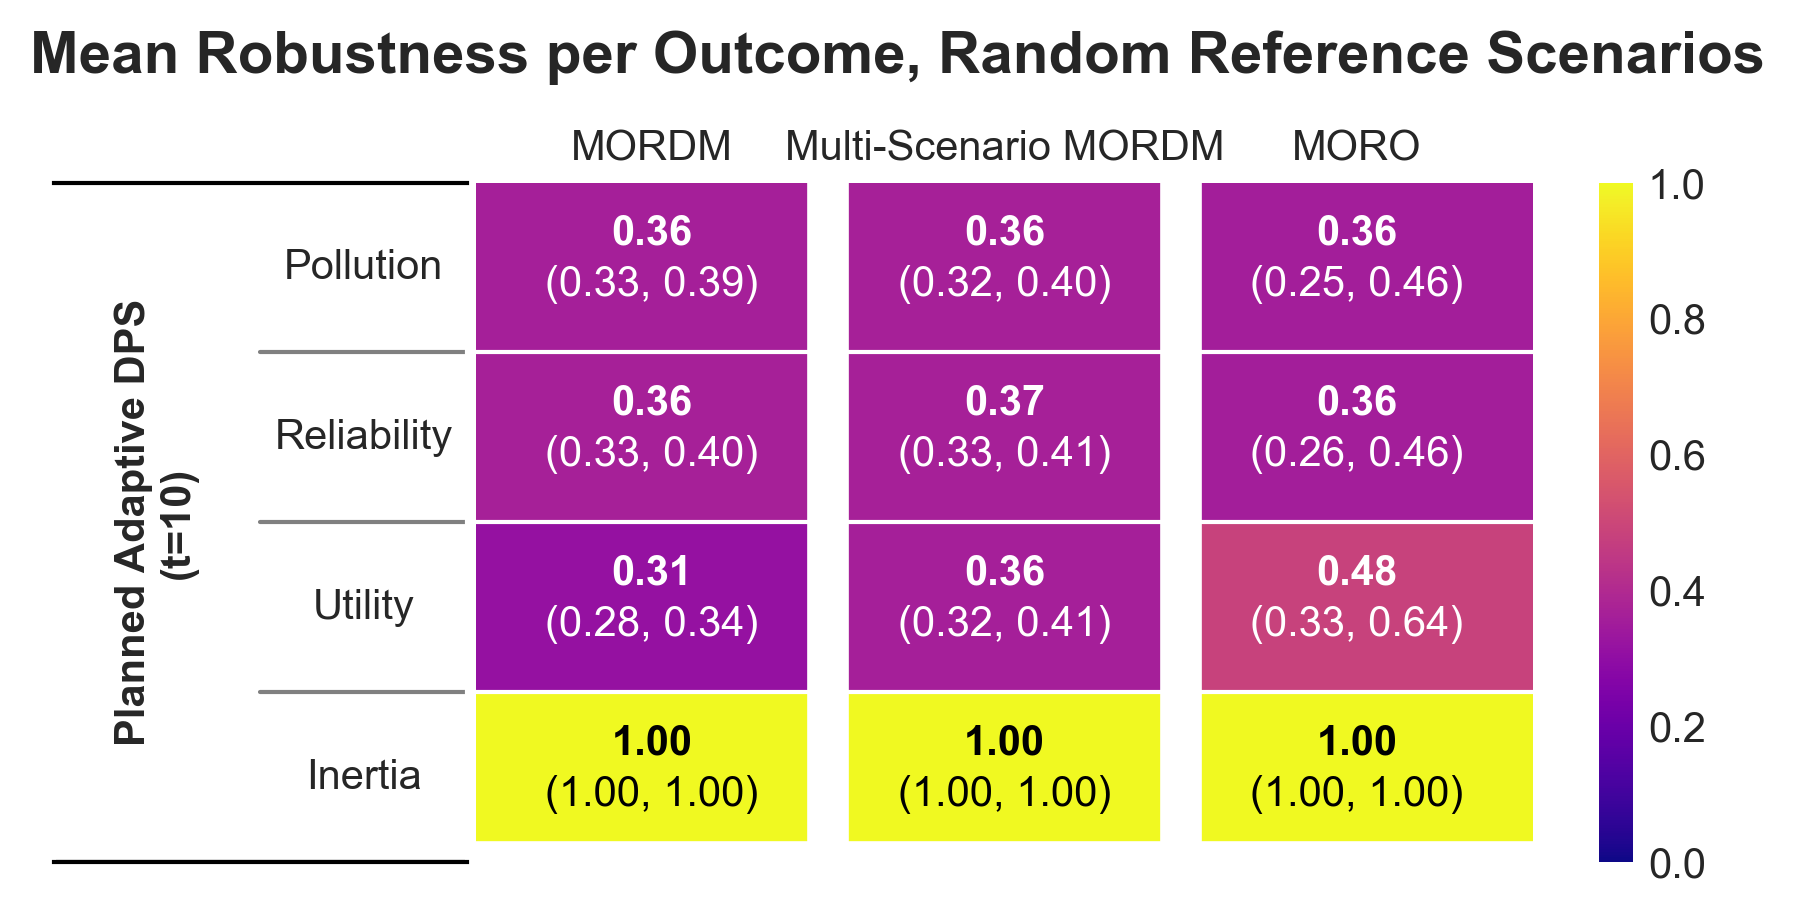
\includegraphics[width=0.85\textwidth]{compare/robust_heatmap_plannedrandom}
        \caption[Mean robustness for planned adaptive variation given random reference scenario selection]{Mean robustness for the planned adaptive DPS problem variation, where multi-scenario MORDM involves the use of a random set of 5 policies.}
        \label{fig:robust-heatmap-planned-random}
    \end{figure}

    \begin{figure}[H]
        \centering
        \captionsetup{width=\textwidth}
        
        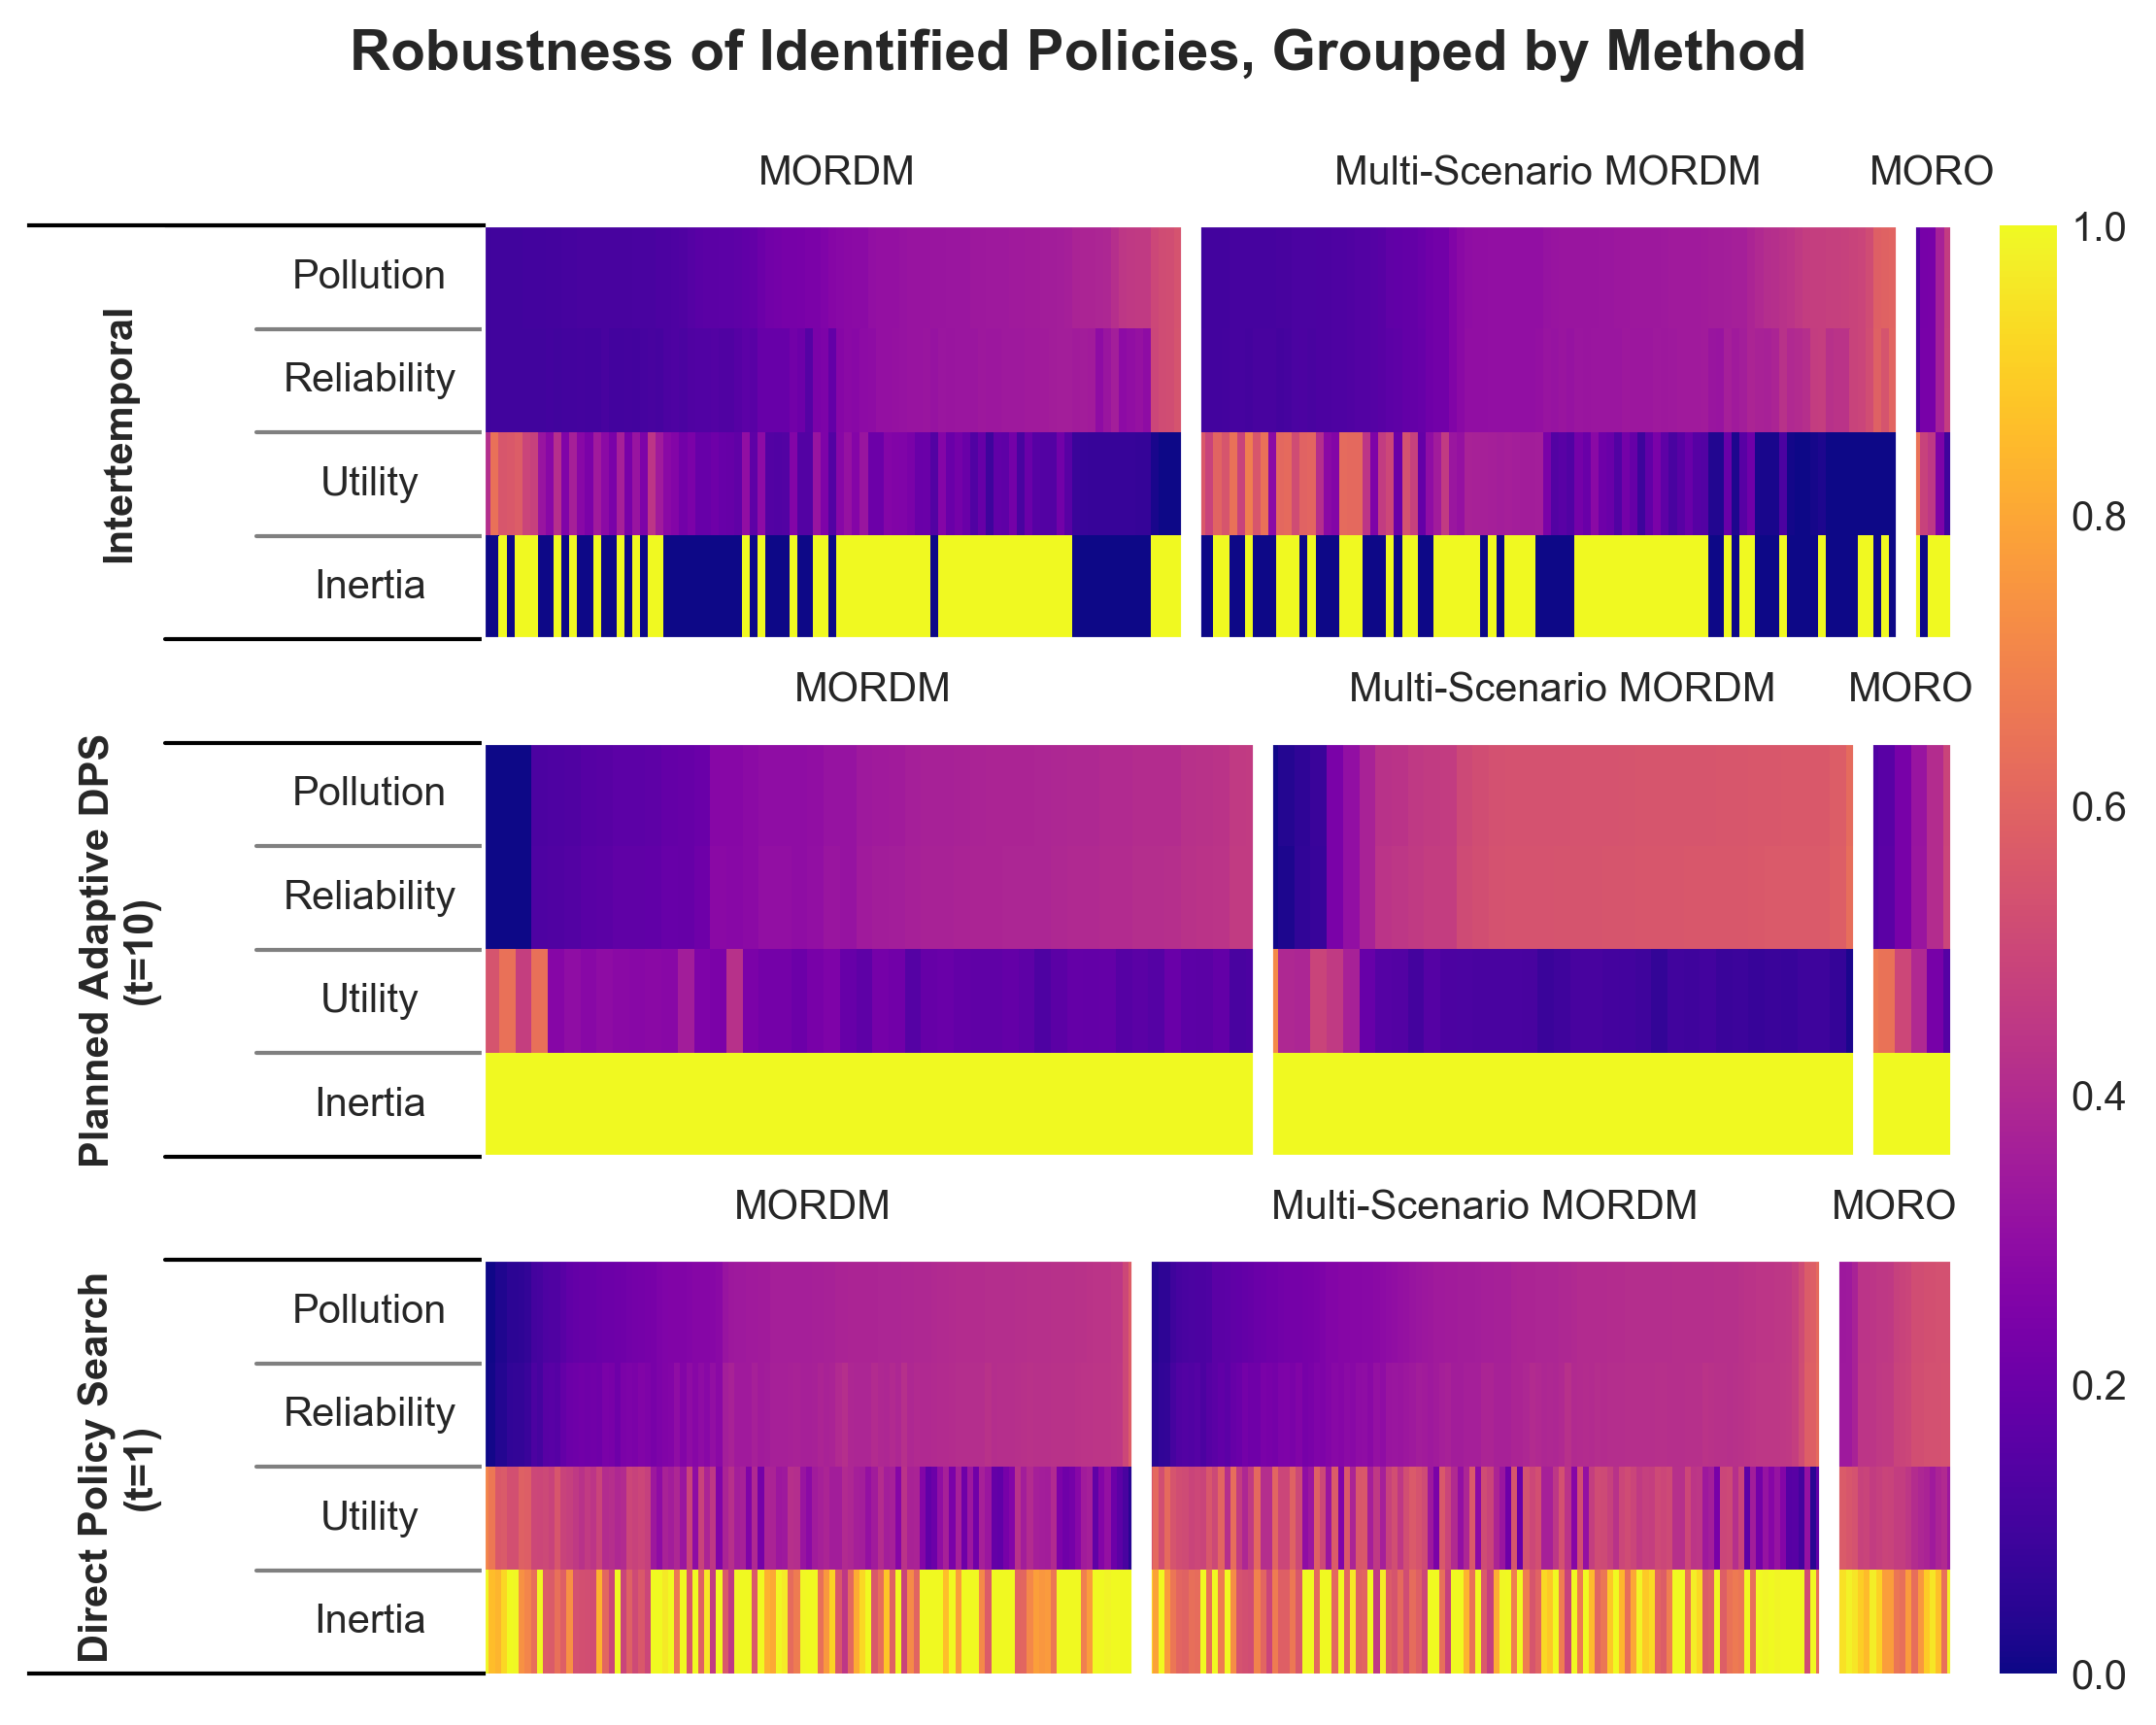
\includegraphics[width=\textwidth]{compare/perpolicyrobustness}
        \caption{Robustness of each outcome of interest per policy in a non-dominated set of alternatives.}
        \label{fig:perpolicy-robustness}
    \end{figure}

    \begin{figure}[H]
        \centering
        \captionsetup{width=\textwidth}
        
        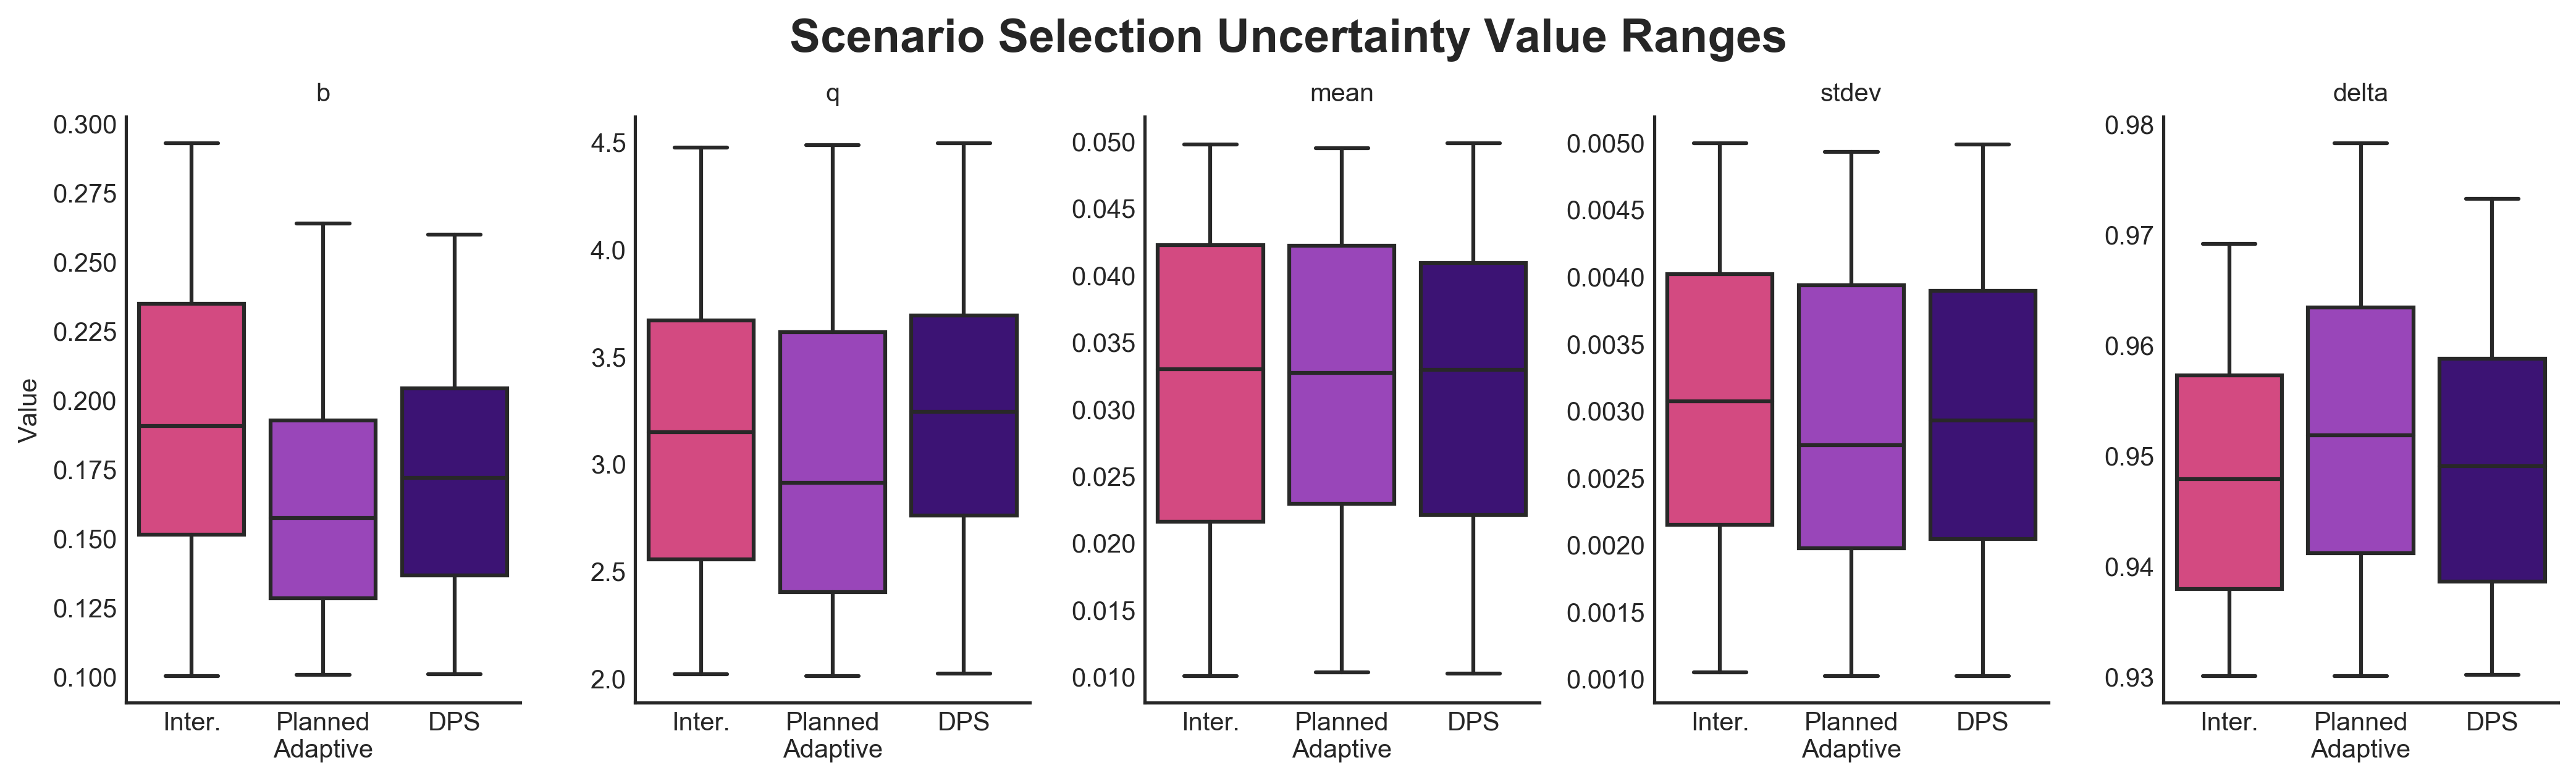
\includegraphics[width=\textwidth]{compare/leverranges_box_scens_highres}
        \caption[Uncertainty value ranges used to select reference scenarios for multi-scenario MORDM]{Ranges of values for each uncertainty parameter that is used to determine a maximally diverse set of 4 policies in the scenario selection process for multi-scenario MORDM.}
        \label{fig:scenarioselect-ranges}
    \end{figure}

    \cref{fig:scenarioselect-ranges} shows the value ranges of each uncertainty parameter that exists in the ensembles of uncertainty vectors that were used to build the sets of 4 maximally diverse policy alternatives for each of the three model variations. This shows that despite the set of reference scenarios for the planned adaptive DPS model variation leading to a set of quite conservative polices, those reference scenarios were selected from a larger ensemble with a relatively similar range of values to the intertemporal and DPS variations. This figure together with the results of the multi-scenario MORDM analysis of the different model variations may indicate that a multi-scenario MORDM analysis of a problem with a policy architecture similar to the planned adaptive DPS, which does not adapt as quickly is more strongly influenced by the reference scenarios selected than the other variations which do. 
    
    The existence of conservative policies with respect to pollution level, which also appears to negatively impacts utility-based robustness, also seems to have had an impact on the diversity of robust outcomes, which provides decision makers with less room for examining the trade-offs that exist when considering a problem with conflicting objectives. As \cref{fig:perpolicy-robustness} indicates, the multi-scenario MORDM analysis of the planned adaptive DPS lake problem does not offer as many policy alternatives that have higher utility robustness and lower pollution and reliability robustness when compared to every other pairing. 

    Also of note in \cref{fig:robust-heatmap-mean} with respect to the planned adaptive DPS model variation is that an increase in robustness of pollution and reliability is not seen in the MORO-based analysis with respect to the MORDM-based analysis, which contrasts with the intertemporal and DPS model variations. This is paired with an increase in robustness of utility for the town, which indicates that while the MORO-based analysis was not able to discover policies that yield a more robust policy with respect to pollution release, it was able to discover policies that maintain a similar level of robustness there while at the same time increasing utility to the town. 
    
    \begin{comparisonbox}{Summary: Robustness of recommended policy set}
        In general, the recommended policy set yielded more robust alternatives the more robustness was incorporated into the search phase of a method, with MORDM yielding the least robust options and MORO the most robust. The exception to this finding is with a multi-scenario MORDM analysis of the planned adaptive model variation. In this case, the policies identified were much more conservative and therefore robust with respect to pollution release and reliability, leading to lower effectiveness for the utility of the town. 
    \end{comparisonbox}
    
    \subsection{Comparison \thecomparison : Similarity of recommended policy sets} \stepcounter{comparison}
    Similarity is examined within method-generated sets of non-dominated policies and is defined as described in \cref{compare-policysimilarity}. The distribution of similarity values for both options, where each value represents the Euclidean distance between two policy alternatives, can be found in \cref{fig:lever-similarity}. 

    \begin{figure}[ht]
        \centering
        \captionsetup{width=0.9\textwidth}

        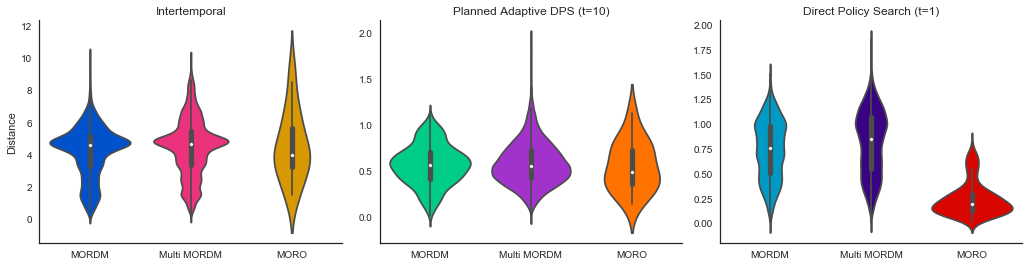
\includegraphics[width=\textwidth]{compare/lever_similarity_within}
        
        \caption{Similarity of lever values, determined between policies of the same method.}
        \label{fig:lever-similarity}
    \end{figure}
    
    \begin{figure}[ht]
        \centering
        \captionsetup{width=\textwidth}
        
        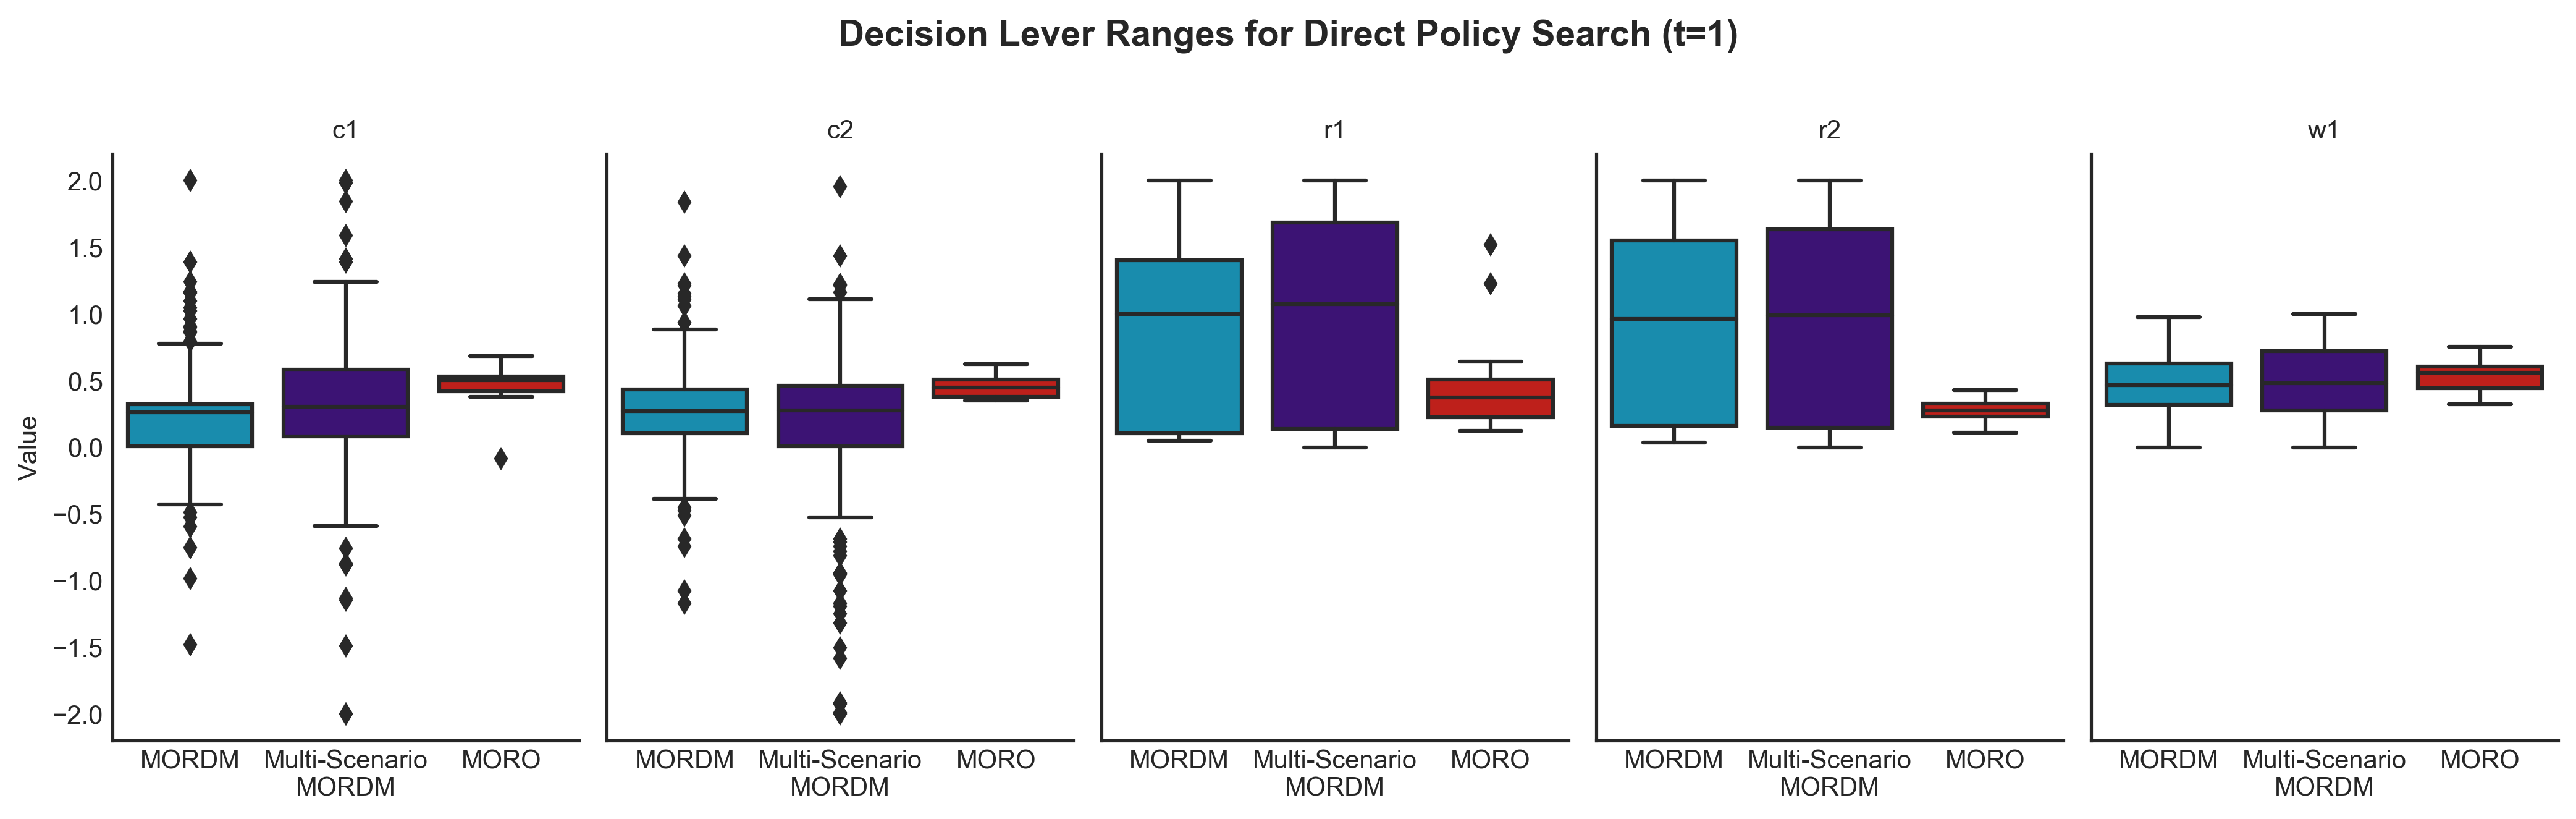
\includegraphics[width=\textwidth]{compare/leverranges_box_dps_highres}
        \caption{Ranges of values for each lever in the non-dominated policy set for the DPS model variation.}
        \label{fig:dps-lever-variation}
    \end{figure}

    \cref{fig:lever-similarity} shows the similarity of sets of policy alternatives to other policies in the same set. A smaller mean distance value, indicated by the white dot in each violin plot element. This chart indicates that there is fairly consistent similarity of policy alternatives within the intertemporal and planned adaptive DPS problem variations. A note within the pairing of the planned adaptive DPS variation and multi-scenario MORDM is the long tail on the upper part of the plot. This indicates that the multi-scenario MORDM method uncovered a small number of policies that are less similar than other policies in the set, given the larger distance value.

    There is an indication that the set of non-dominated policy alternatives generated for the DPS lake problem through MORO results in a less diverse policy set, due to the significantly smaller mean distance values shown in \cref{fig:lever-similarity}. This indicates that decision makers will have a less diverse set of options to work with, which may prove problematic as decision makers seek to balance conflicting objectives. This is born out in \cref{fig:dps-lever-variation}, which shows the ranges of values for each decision lever for the DPS model variation found with each method. With this plot, it is clear that the MORO analysis produces polices from a smaller range of values for each decision lever. At the same time, as seen in \cref{fig:robust-heatmap-mean}, a greater robustness was achieved for each of the outcomes of interest for the DPS + MORO pairing, indicating that despite MORO uncovering a less diverse set of policy alternatives, that set of alternatives is more robust overall, providing a stronger set of alternatives to decision makers for further analysis and development. 
    
    \begin{comparisonbox}{Summary: Similarity of recommended policy sets}
        Save a two identified exceptions, each method is produces sets of policy alternatives with fairly consistent similarity. The multi-scenario MORDM analysis of the planned adaptive DPS variation produces a small number of outlier policies that are less similar than the large majority of policies in that set. Finally, the MORO analysis of the DPS problem variation produces a significantly less diverse set of alternatives, but that set of alternatives is still able to produce a higher level of robustness than is found with the other two methods. 
    \end{comparisonbox}
    
    \subsection{Comparison \thecomparison : Similarity of robustness values} \stepcounter{comparison}
    The final point of comparison considers the similarity of robustness values given a set of similar policies. The purpose of this metric is to determine how robustness is reported for similar policies, to establish a better frame of reference for comparing robustness values of the different methods being studied. In the case of this research, the robustness measure is defined in an identical manner for all three methods. Therefore, the robustness values are directly comparable across method and model parings, and identical policies identified with different methods and tested against the same ensemble of uncertainty vectors in the computational exploration phase will result in identical robustness values. 
    
     \begin{comparisonbox}{Summary: Convergence of search}
        Because all three methods under consideration use the same robustness metric and share a common parameterization of that metric, robustness values will be the same for identical policies found with different methods. 
    \end{comparisonbox}
        